\section{Câu 14}

Cho 3 dạng sóng 1 $v_1(t)$, $v_2(t)$ và $v_3(t)$ như hình vẽ. Thiết kế mạch biến đổi sử dụng
OPAMP có 2 ngõ vào là $v_1(t)$, $v_2(t)$, mạch cho ngõ ra là dạng sóng $v_3(t)$. Giả sử
OPAMP sử dụng là lý tưởng.
\begin{figure}[H]
	\centering
	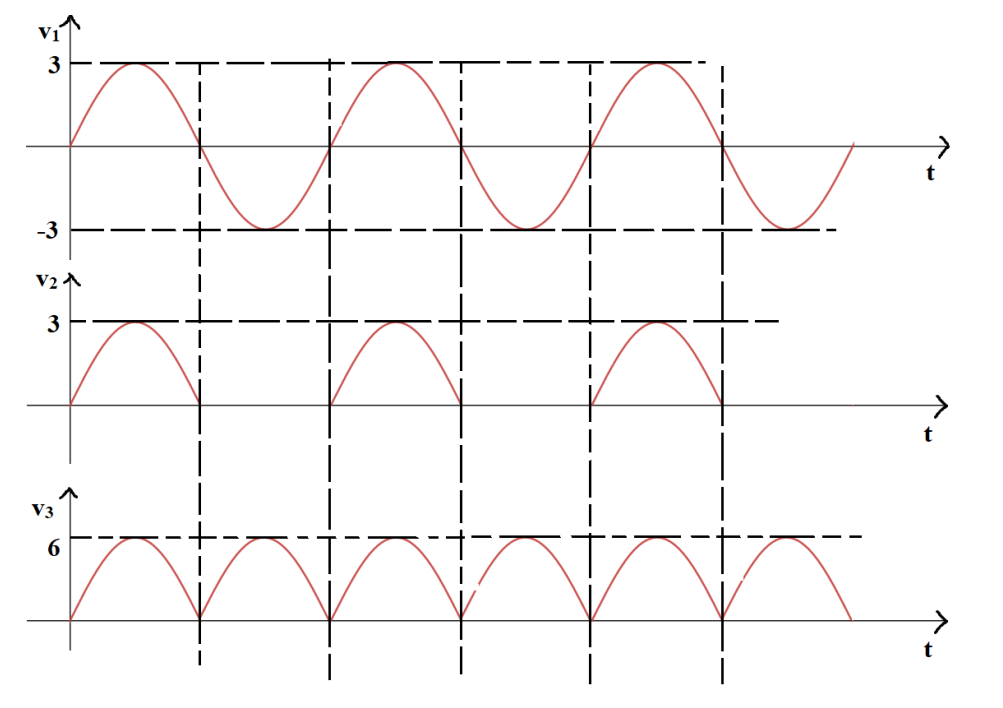
\includegraphics[scale=0.9]{image/C14_De.png}
\end{figure}
\begin{center}
\textbf{Bài giải}
\end{center}
$v_1(t)$ đi qua mạch Negative Half Cycle để lấy phần âm. Sau đó đi qua mạch cộng để kết hợp với $v_2(t)$.
Cuối cùng qua mạch khuếch đại đảo để có $v_3(t)$.\\

\begin{figure}[H]
	\centering
	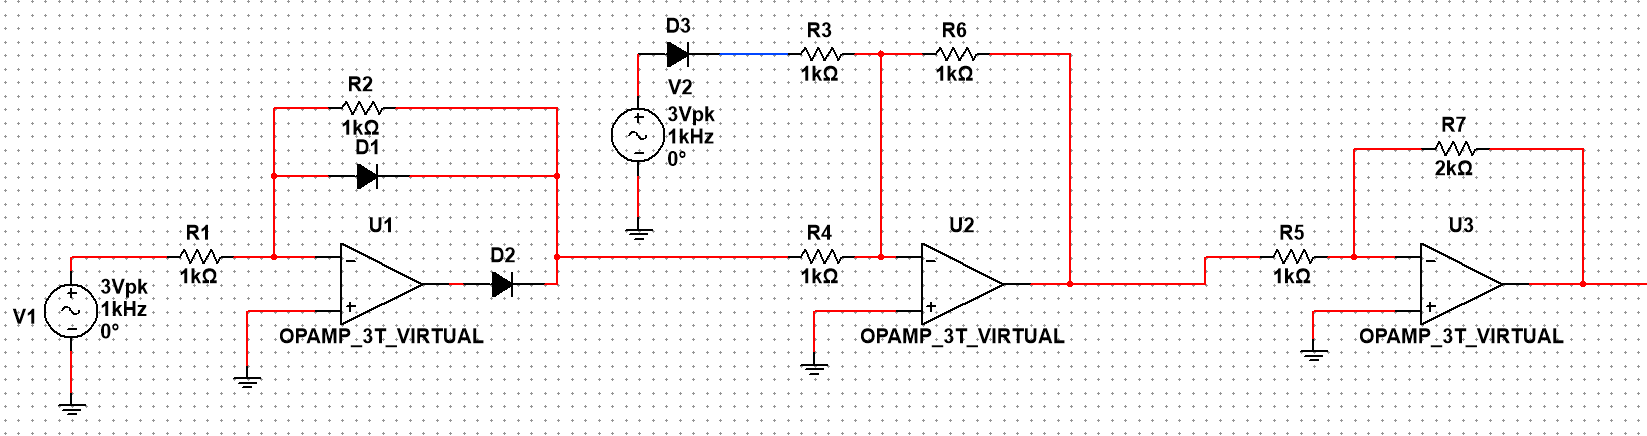
\includegraphics[scale=0.5]{image/C14_BT.png}
\end{figure}

Vì tầng 1 và 2 biên độ điện áp không đổi nên các điện trở chọn bằng 1k$\Omega$.
Tại ngõ ra của tầng 2, sẽ là tín hiệu âm của $v_1$ cộng với $v_2$ nhưng bị đảo và có biên độ điện áp là -3V.
Chính vì thế cần qua 1 bộ khuếch đại đảo với độ lợi bằng 2 để có $v_3$. Chọn R5=1k$\Omega \rightarrow$ R7=2k$\Omega$.

\begin{figure}[H]
	\centering
	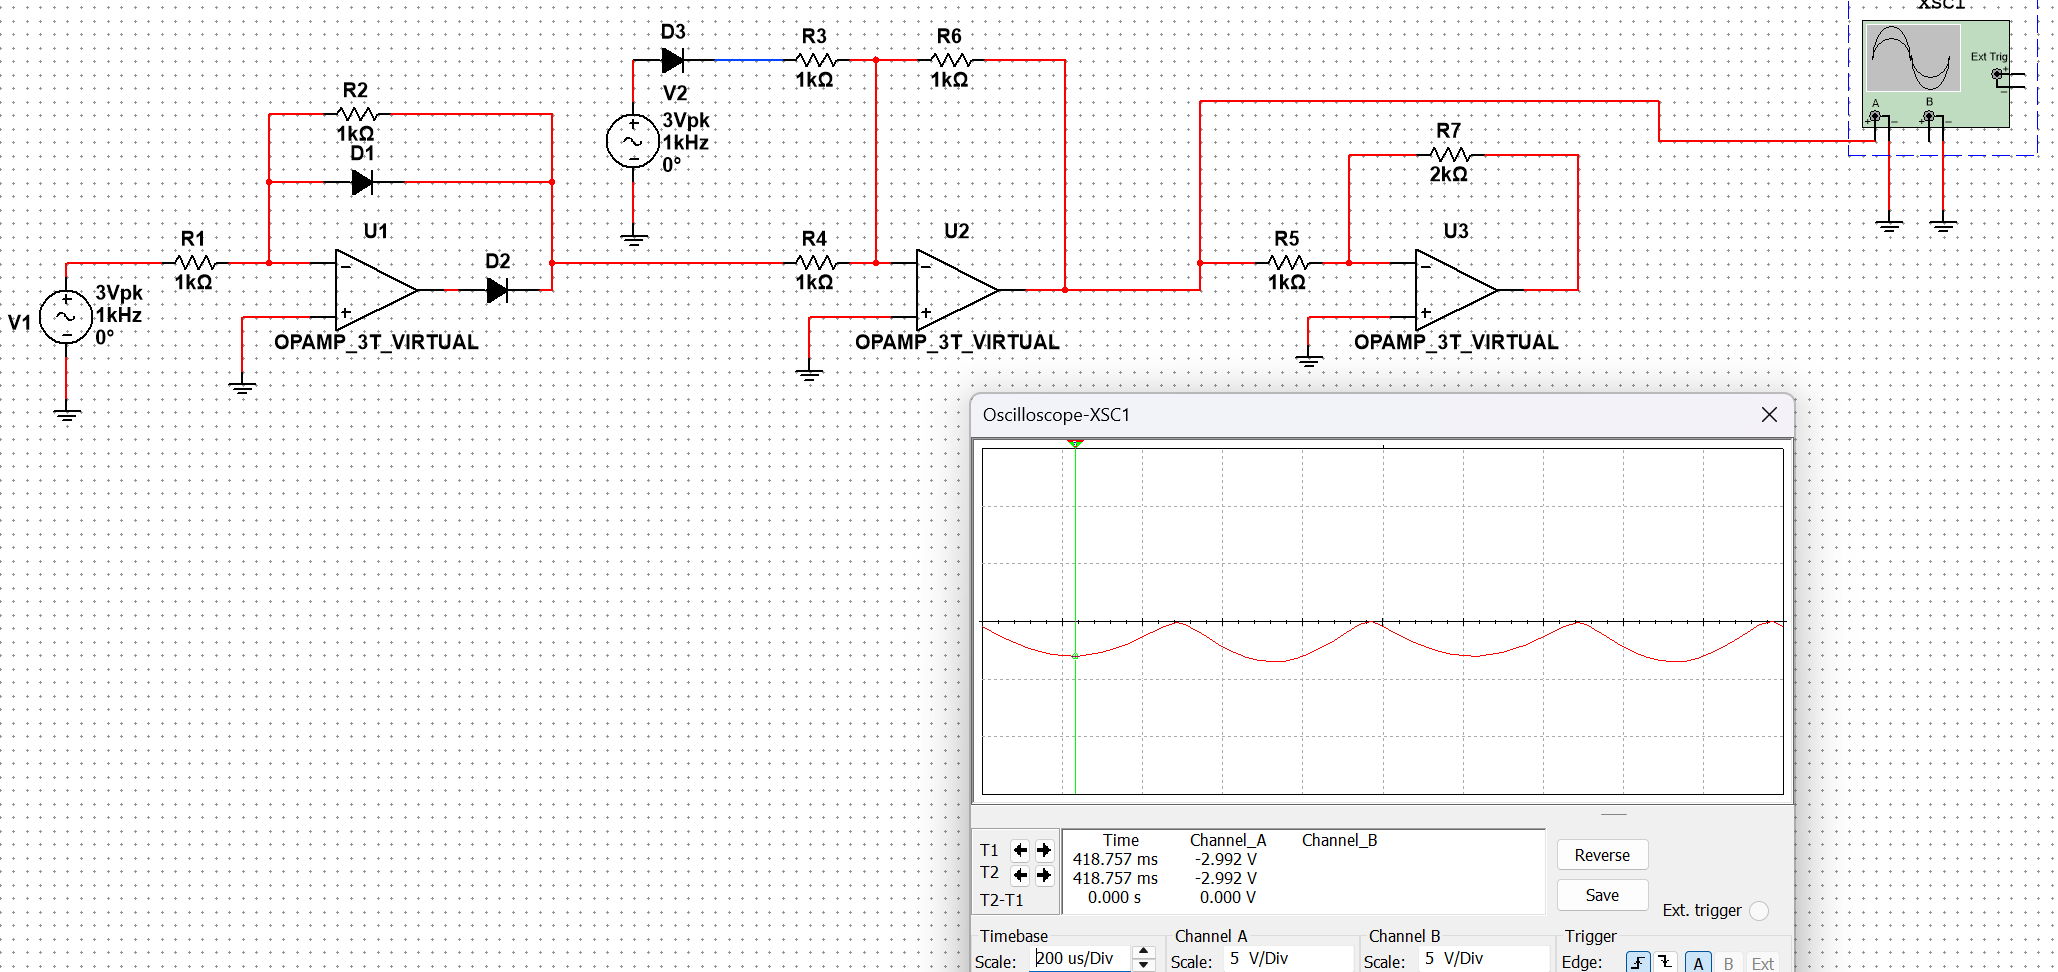
\includegraphics[scale=0.45]{image/C14_vo2.png}
    \caption*{Hình 1. Ngõ ra tại tầng 2}
\end{figure}
\begin{figure}[H]
	\centering
	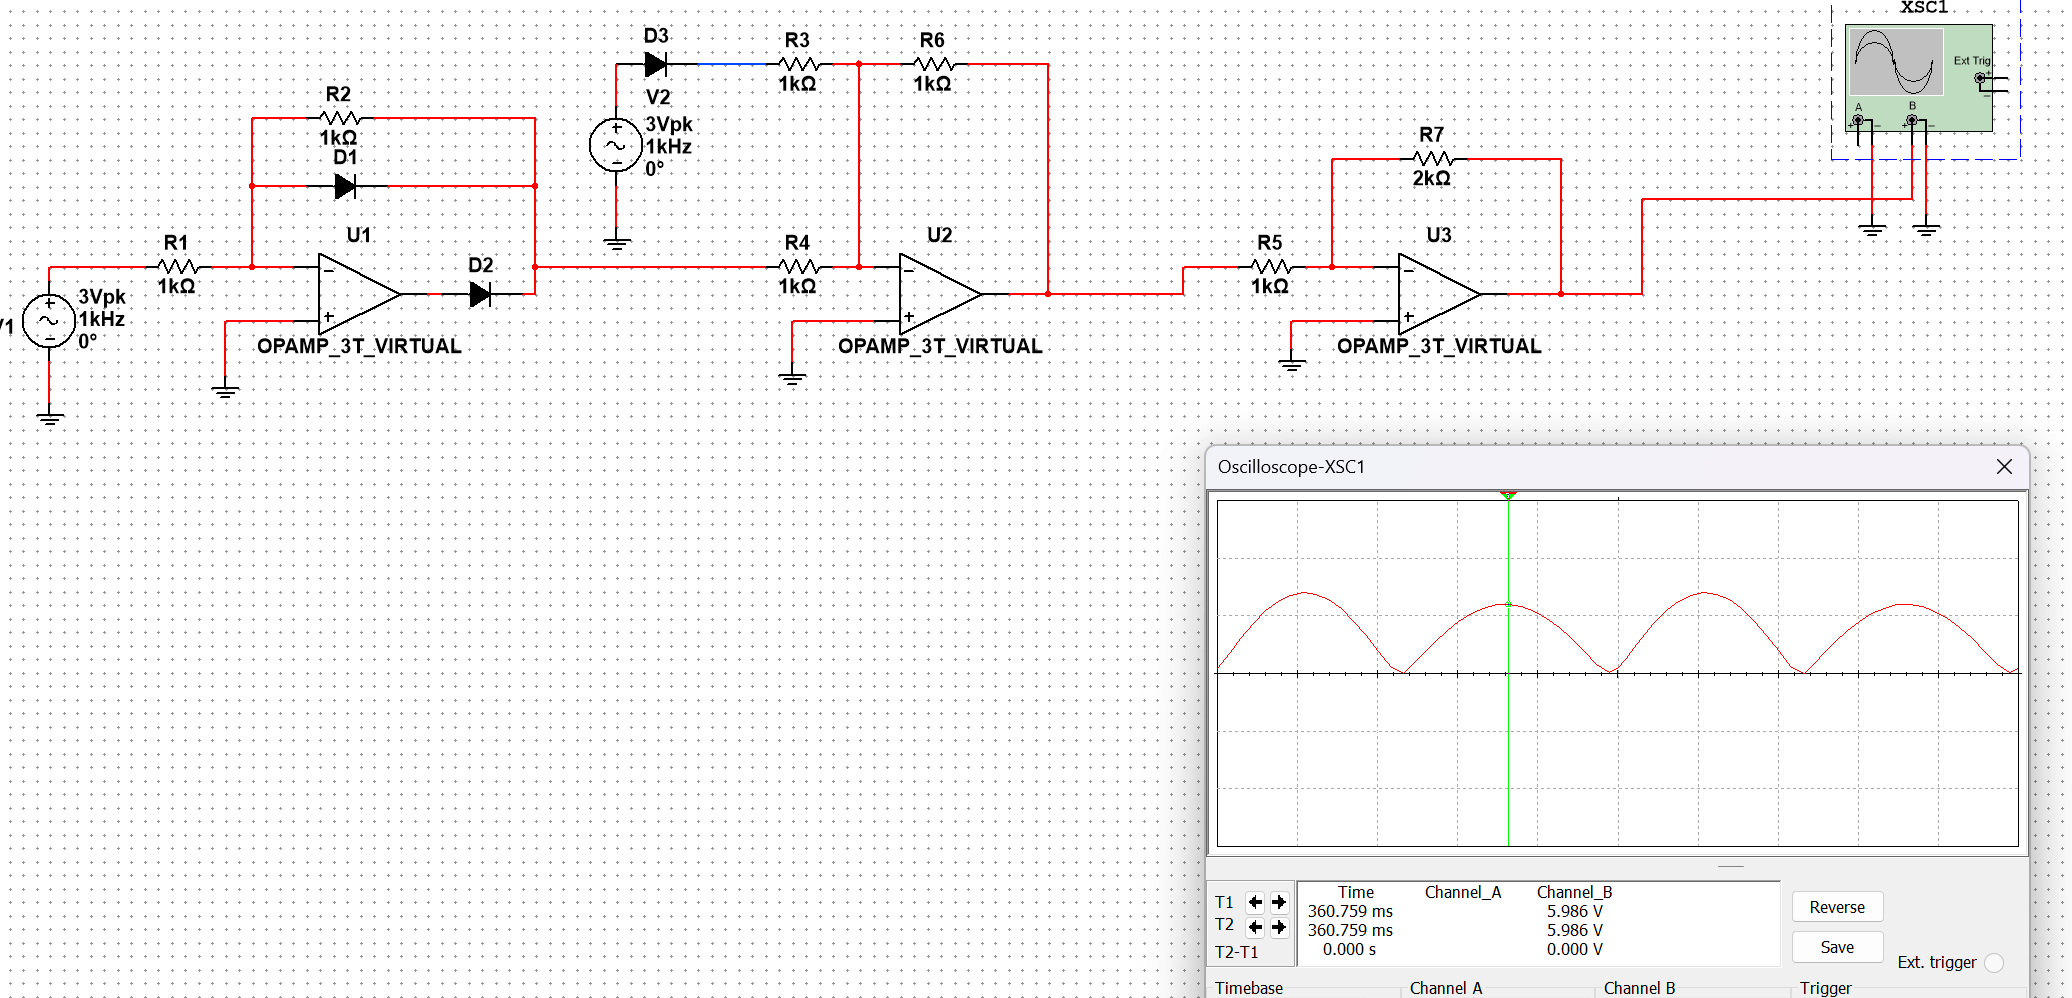
\includegraphics[scale=0.45]{image/C14.png}
    \caption*{Hình 2. Ngõ ra của mạch}
\end{figure}
\textbf{Nhận xét:}\\
- Hình 1: Có thể thấy ngõ ra tại tầng 2 có biên độ điện áp là -2.992V xấp xỉ với -3V đã tính ở trên.\\
- Hình 2: Ngõ ra của mạch có biên độ điện áp là 5.986V xấp xỉ 6V với yêu cầu đề bài.
